\documentclass[a4j,11pt]{jarticle}
%\usepackage{epsfig,here}
\usepackage{url}
\usepackage{here}
\usepackage{listings}
\usepackage{comment}
\usepackage[dvipdfm]{hyperref}
\usepackage[dvipdfmx]{graphicx}
\usepackage{mediabb}
\usepackage{moreverb}
\setcounter{secnumdepth}{5}
\setlength{\textwidth}{1.1\textwidth}
\setlength{\oddsidemargin}{-3pt}
\setlength{\evensidemargin}{\oddsidemargin}
\setlength{\topmargin}{10mm}
\setlength{\headheight}{0mm}
\setlength{\headsep}{0mm}
\begin{document}
\begin{center}
%\noindent
\vspace{10mm}
{\bf {\huge 研究プロジェクト後半 秋山研究室 レポート}}\\
%\end{center}
\vspace{80mm}
提出日:2021年5月28日\\
\vspace{10mm}
系:情報工学系\\
\vspace{10mm}
学籍番号:19B12223\\
\vspace{10mm}
\vspace{20mm}
{\bf {\LARGE 氏名:玉野 史結}}
\end{center}
\newpage
\section{1-A) イブプロフェン構造式}
%作成したプログラムを提示し、プログラムの内容や、工夫した点について説明せよ。
\begin{figure}[H]
\centering
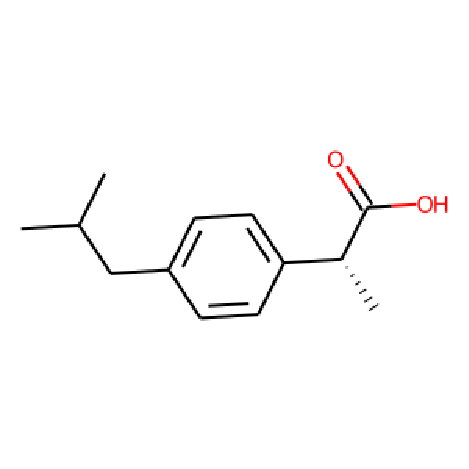
\includegraphics[scale=0.5]{./images/exercise_A_Ibuprofen.pdf}
\caption{実習1-A イブプロフェンの構造式出力}
\label{fig:ex1_A}
\end{figure}

\section{1-D)  $\ln{K_a}$ 値を計算する関数の設計}
%作成したプログラムを提示し、プログラムの内容や、工夫した点について説明せよ。
Tajimiらの論文~\cite{paper1_Tajimi}によると,Supplementary Table S1.に含まれる $f_b$ 値は実数値のものもあれば $f_{bmin}-f_{bmax}$ のように範囲で指定されているものもある。範囲指定されている場合には\\
\linebreak
\centerline{$f_b = \frac{f_{bmin} + f_{bmax}}{2}$}\\
\linebreak
としたと記述されている。また\\
\linebreak
\centerline{$\ln{K_a}=C\ln{\frac{f_b}{1-f_b}}$}\\
\linebreak
と定義されており,定数 $C$ は先行研究~\cite{C_previous}より$0.3$と設定,また $\ln{K_a}$ 値の発散を防ぐため $f_b$ は $f_b\times0.99+0.005$ としていた。\par
そのため,関数 \texttt{calc\_lnka(fb)} の最初のステップは,引数 \texttt{fb} に対してまずデータのタイプが \texttt{float} であるか否かを確認し,さらに「\texttt{-}」で区切った時のリストの長さが1より大きいかを確認することとした。 \texttt{float} でなく,かつ区切ったときのリストの長さが1よりも大きい場合, $f_b$ は範囲で指定されているということになるため,リストの1つ目の要素(\textit{i.e.}  $f_{bmin}$ )とリストの2つ目の要素(\textit{i.e.}  $f_{bmax}$ )の平均をとったものを $f_b$ とした。当てはまらない場合は値が与えられているため $f_b$ の値はそのままである。その後, $f_b$ の値に $0.99$ を乗算し $0.005$ を加算することによりスケーリングを行なった。\par
このようにして得られた $f_b$ を \texttt{scaled\_fb} と表現することとし,関数の出力を,\\
\linebreak
\linebreak
\centerline{$0.3\times\ln(\frac{\texttt{scaled\_fb}}{\texttt{1-scaled\_fb}})$}
\linebreak
\linebreak
として関数を定義した。

\section{1-E) 学習器に Lasso 回帰を用いた際のハイパーパラメータ等について}
ここでは,以下の5点について記述する。\\
\begin{itemize}
\item 最適化したハイパーパラメータ
\item 各ハイパーパラメータの探索範囲
\item ハイパーパラメータ探索方法
\item 最良ハイパーパラメータ
\item 最良ハイパーパラメータにおける cross validation 中の $\ln{K_a}$ 値の RMSE と $\ln{K_a}$ 値の相関係数 R 
\end{itemize}

\subsection{最適化したハイパーパラメータ}

\texttt{sklearn.linear\_model.Lasso}におけるパラメータおよびその意味は,以下である。~\cite{sklearn_Lasso}

\begin{itemize}
\item \textit{alpha}\\
 \textit{alpha} はラグランジュ乗数を表しており,以下の式の第2項の係数となっている。overfitting を抑制する効果がある一方,大きすぎると underfitting 問題が発生するため,最適化の必要があると考えた。\\
 \linebreak
$$\frac{\|y - Xw\|_2^2}{2\times n} + \textit{alpha}\|w\|_1 \eqno(1)$$\\
 \linebreak
 なお, $y$ は真値, $Xw$ は予測値, $w$ は重み, $n$ はサンプル数を表す。
\item \textit{fit\_intercept}\\
 \textit{fit\_intercept} は切片を計算するか否かを決める \textit{bool} 値である。データが原点を通る直線でプロットされることが確実である場合には \textit{False} で良いが,本課題では default 値でもある \textit{True} とした。 
\item \textit{normalize}\\
 \textit{normalize} は正規化を行うか否かを決める \textit{bool} 値である。本課題では,説明変数に標準化を施すのみで,正規化は行わずに進めることとした。従って,本課題では default 値でもある \textit{False} とした。
\item \textit{precompute}\\
 \textit{precompute} は計算速度を高めるためにグラム行列を用いるか否かの指標である。 本課題では標準化を行った後に学習させるため,グラム行列は相関行列となる。 \textit{sparse input} であればスパース性の保持のため \textit{False} となるが,本課題では \textit{sparse input} でない上に,用いる必要がないと判断し \textit{True} とした。
\item \textit{copy\_X}\\
 \textit{copy\_X} は overwrite を行わないか否かを決める \textit{bool} 値である。本課題では,\textit{True} とし, overwrite を行わないようにした。
\item \textit{max\_iter}\\
 \textit{max\_iter} は iteration の回数を指定するパラメータである。最適化する必要があると考えた。
\item \textit{tol}\\
 \textit{tol} は(1)式の最適化をどの程度寛容するかを表す指標である。この値よりも小さくなるまでイテレーションが行われる。最適化の必要があると考えた。
\item \textit{warm\_start}\\
 \textit{warm\_start} は前回学習させた学習器の情報を再利用するか否かの指標であり,本課題では平等に評価を行うために \textit{False} とした。
\item \textit{positive}\\
 \textit{positive} は係数を正とするか否かの指標であるが,本課題では係数が負の場合も十分にありうると考え,default 値でもある \textit{False} とした。
\item \textit{random\_state}\\
 \textit{random\_state} は以下で説明する\textit{selection}が \textit{random} の際に,どのような擬似乱数に基づいて係数選択を行うかを指定する。本課題では \textit{cyclic} を用いたため,このパラメータは設定しなかった。
\item \textit{selection}\\
 \textit{selection} は \textit{random} か \textit{cyclic} をとるパラメータであり,回帰における係数の設定方法について指定する。 \textit{random} は特に, \textit{tol} が 1e-4よりも大きい場合に収束が早くなる。後述するが,本課題では\textit{tol} の探索範囲を 1e-6 から 1e-4 としたため,このパラメータは default 値の \textit{cyclic} とした。
\end{itemize}

以上より,最適化するハイパーパラメータは \textit{alpha} , \textit{max\_iter} , \textit{tol} の3つとした。

\subsection{各ハイパーパラメータの探索範囲}

\begin{itemize}
\item \textit{alpha}\\
 \textit{alpha} が大きくなればなるほどパラメータの複雑さ(\textit{i.e.} (1)式の$\|w\|_1$)が与える影響が大きくなる一方で,モデルのデータへの適合具合が軽視されることになる。default 値では $1.0$ のため,本課題では \textit{alpha} の探索範囲を 1e-2 から $1.5$ まで探索を行い,適切な \textit{alpha} を求めた。\\
\item \textit{max\_iter}\\
 \textit{max\_iter} は,\textit{tol}を 適切に設定すれば比較的重要性が低いと考え, default値が $1000$ であるため,$1000$ から $100000$ までとした。
\item \textit{tol}\\
 \textit{tol} は default では 1e-4 であるが, \textit{alpha} の値を1e-2から$1.5$までと, default 値よりは平均してやや小さくなる値でとっているため,寛容性を低くしても良いと考え,値を小さくし,1e-6から1e-4に設定した。
\end{itemize}

\subsection{ハイパーパラメータ探索方法}
今回の課題においてハイパーパラメータ探索には optuna\cite{optuna}を用いて, cross validation における RMSE 値の平均をとり,その値が最小となるように100回探索を行った。 
\subsection{最良ハイパーパラメータ}
探索を行った3つに対し,最良ハイパーパラメータは以下のようになった。\\
\linebreak
$\textit{alpha} = 0.010001550247043559$\\
$\textit{max\_iter} = 18633$\\
$\textit{tol} = 2.0186369425523876$e-$05$\\
\subsection{最良ハイパーパラメータにおける cross validation 中の $\ln{K_a}$ 値の RMSE と $\ln{K_a}$ 値の相関係数 R}
 cross validation 中の $\ln{K_a}$ 値の RMSE 並びに $\ln{K_a}$ 値の相関係数 R を以下に示す。\\
\begin{itemize}
\item  cross validation 1\\
RMSE $= 0.5209547078388901$\\
R $= 0.7107256587155896$ \\
\item  cross validation 2\\
RMSE $= 0.4606982018660353$\\
R $= 0.7605366763431665$ \\
\item  cross validation 3\\
RMSE $= 0.4281213900359186$\\
R $= 0.7542478496501217$ \\
\item  cross validation 4\\
RMSE $= 0.49896753871626187$\\
R $= 0.7249485193449345$ \\
\item  cross validation 5\\
RMSE $= 0.4763822826075803$\\
R $= 0.7516799440924689$ \\
\end{itemize}

\section{1-F)  Cyclic peptide drug の予測における $\ln{K_a}$値の RMSE , $\ln{K_a}$ 値の相関係数 R}
 1-E で選択されたハイパーパラメータを用いて Small molecule データを教師データとした Lasso 回帰でCyclic peptide drug の予測を行なった結果を以下に示す。\\
 \linebreak
RMSE $= 891905781196.9539$\\
R $= -0.16718436183577068$ \\
\section{1-G) E)とF)の予測精度の比較・考察}

予測精度は F)で得られたものの方が低かった。 Lasso 回帰は線形回帰であるため,予測値が真値より一定値離れてしまうことは考えられるが,その点を考慮しても大幅に真値と離れているものが存在し,それらは $\ln{K_a}$ を非常に小さい値であると予測していた。テストデータにおける説明変数を確認したところ,\textit{Ipc}という記述子に対してのみ非常に大きな値をとっており,重みは$-0.018062564152947512$であったことから,この記述子が外れた予測に影響していると考えた。それぞれの値を以下に示す。
\begin{itemize}
\item  Acetyl-Daptomycin\\
 $\textit{Ipc} = 1.90252689$e+$03$\\
 $\ln{K_a} = -0.5870781$\\
 $prediction = -3.50131812$e+$01$\\

\item  Daptomycin\\
 $\textit{Ipc} = 1.20007563$e+$06$\\
  $\ln{K_a} = 0.51222289$\\
 $prediction = -2.16764776$e+$04$\\

\item  Telavancin\\
 $\textit{Ipc} = 1.03358327$e+$11$\\
  $\ln{K_a} = 0.63662153$\\
 $prediction = -1.86691641$e+$09$\\

\item  Dalbavancin\\
 $\textit{Ipc} = 2.41744875$e+$14$\\
  $\ln{K_a} = 0.75673178$\\
 $prediction = -4.36653231$e+$12$\\

\item  Oritavancin\\
 $\textit{Ipc} = 8.80504378$e+$12$\\
  $\ln{K_a} = 0.51222289$\\
 $prediction = -1.59041668$e+$11$\\
 
\end{itemize}

予測値の値の大小と \textit{Ipc} の値の大小が関係していることから, \textit{Ipc} が誤った予測に関与していることは間違いないと考える。この \textit{Ipc} 値が異常に大きくなることは Github の issue にてあげられていた。\cite{git_ipc} これによると,\texttt{avg=True} とすれば良いと書かれており,改めて 2D記述子 を並べたベクトルを構成する関数を作り変えた。考察段階で \textit{Ipc} という記述子は \texttt{Descriptors.descList} において index が 40 であることが分かっていたため,その値のみ再び \texttt{avg=True} という引数を加えて再計算した予測値が以下となった。\\
\linebreak
RMSE $= 0.7231702603632365$\\
R $= 0.4526782165593785$ \\

並外れた値では無くなったが,やはり Cyclic peptide drug に対する予測精度の方が低かった。
修正後の 2D記述子 を用いて計算を行った結果,真値との差を確認すると,ある分子に対して大きく外れているというわけではなかったが,誤差の平均を計算すると$0.15672424808532037$となり,全体として $\ln{K_a}$ 値をやや小さく予測していることが分かった。 Cyclic peptide は Small molecule と比較すると大きな分子であり,立体構造による影響がより大きくなる一方で 2D 記述子では平面的な構造の数値化しか行えていないためにこのような予測制度になっていると考えた。

\section{1-H) 重要な記述子についての考察}
重要な記述子を Lasso 回帰において係数の絶対値が$0.075$より大きいものであると定義する。その時,重要な記述子は RDKit の 2D descriptors $208$ の内,$6$に絞られた。それらを係数の絶対値の大きいものから順に示す。\\

\begin{itemize}
\item  \textit{MolLogP} (weight : $0.2846387781835837$) \\
 \textit{MolLogP} はWildman-Crippen LogP 値を表している。\cite{rdkit_mollogp} $\log{P}$は分子の有機層と水層中の平衡状態における濃度比率である分配係数 $P$ の対数値であり,大きい値であると有機層における濃度が高いすなわち脂溶性が高いことを示す指標となっている。\cite{logp}  Wildman-Crippen LogP とは Wildman と Crippen が考案した原子単位での $\log{P}$ を計算し,分子を構成する原子を分子内相互作用等も考慮して分類し,その寄与度合を用いて,和をとることで算出される値である。\cite{mollogp}\par
従って,この記述子の重みの絶対値が大きいということは,脂溶性と $\ln{K_a}$ 値,すなわち血漿タンパク質との結合率 $f_b$ との関係が大きいということであり,かつ係数が正であるから脂溶性が大きい程 $\ln{K_a}$ 値が大きくなる,すなわち $f_b$ が大きくなるということが小分子データから学習されていることになる。
\item  \textit{FpDensityMorgan1} (weight : $-0.14901095942588066$) \\
 \textit{FpDensityMorgan1} を考える上で,まず Morgan Fingerprint について考える。Morgan Fingerprint は ECFPに相当するものであり,原子からの一定結合距離にある部分構造を数えていくものである。\cite{fp}また,その距離 (radius) は2に設定されており, \textit{FpDensityMorgan1} の \textit{1} はソースコードより対象とする環境から取り除く原子の ID であると考えられる。\cite{fp_source1}\cite{fp_source2} すなわち, \textit{FpDensityMorgan1} は ECFP の密度の内,原子 ID が 1 のものを取り除いた指標であると考える。 \par
 この記述子の重みの絶対値が大きいということは,原子から半径2の構造のフィンガープリントが $f_b$ に関与しており,原子 ID が 1 のものを取り除いたものが指標として重要であることが分かった。一方で,原子 ID 1 のものを除去することでどのような恩恵があるのか分からなかったが,\cite{fp_ID}を参考にすると,C 原子に結合している原子が ( C $\times$ 3,  H $\times$ 1 ) の場合に原子 ID が 1 になっていた。参考サイトにおける原子 ID が全分子に共通のものであるとするならば,先述した原子は Fingerprint Densityを計算する上で密度を高くしてしまう,もしくは低く計算してしまい,$f_b$ を予測する上でその影響が比較的大きくなると考えた。
\item  \textit{HallKierAlpha} (weight : $-0.11381840054960113$) \\
 \textit{HallKierAlpha} は Hall と Kier によって提案された指標であり,対象とする原子の共有結合半径と混成軌道の両方の影響をエンコードしたものであり, $sp^3$混成軌道の場合に値が0となる。\cite{hallkier}\par
 従って,この記述子の重みの絶対値が大きいということは,$f_b$ を予測する際には共有結合半径や原子の混成軌道といった指標が重要だと分かり, $f_b$ が血漿タンパク質との結合率であることを考えると,確かに結合においてその半径・混成軌道は重要な指標であると考えられるため学習ができていると考えた。
\item  \textit{fr\_quatN} (weight : $-0.09347316929887078$) \\
 \textit{fr\_quatN} は 窒素原子が電子を 1 つ失った 4 価窒素の数を表している。\cite{fr}\par
 従って,この記述子の重みが負であるということは, 4 価窒素の数が多いとき $f_b$ が小さく予測されることになる。血漿タンパク質は負に荷電している\cite{plusma}ことを考えると正の電荷を帯びている 4 価窒素の数が多い場合には結合しやすくなると考えたが,分子全体として電荷を打ち消しあっていると仮定した場合,局所的に正電荷を帯びている場合には局所的に負電荷を帯びている部分があるということも意味し,負電荷を帯びた部分からは反発力により結合しないと考える。以上より, 4 価窒素を多く有する構造は正電価を帯びた窒素原子は立体的にみた場合に分子の内側,負電荷を帯びた原子がその外側に位置しているのではないかと考える。
\item  \textit{VSA\_EState10} (weight : $0.08555745188948738$) \\
 VSA 記述子は van der Waals surface area 記述子を指し,これは MOE 独自の記述子であり,$\log{P}$,モル屈折,電荷の特性に関し,ある一定の範囲内の分子の表面積を記述子の値として表したものである。\cite{moa_vsa} \textit{VSA\_EState} は特に置換基や官能基による寄与を,表面積の寄与を bin として作成したものであり,\textit{VSA\_EState10} は記述子の値が $11.00$ 以上のものを指す。\cite{estate_vsa}なお,似た記述子に \textit{EState\_VSA} があり,これは置換基や官能基による寄与を bin として表面積の寄与の値を取ったものである。\par
 この記述子の重みが大きいということは置換基や官能基の寄与が大きい場合には $f_b$ が大きくなると予測されており,結合という観点から考えると,置換基・官能基による障害は確かに影響をもたらしていると考えられる。そのため,学習が適切に進んだと考える。
\item  \textit{qed} (weight : $0.07588883863605525$) \\
 \textit{qed} は薬らしさを 771 個の傾向医薬品データセットを用いて定量化したものとなっており,分子量,$\log{P}$,水素結合ドナーの数,水素結合アクセプターの数,極性表面積,回転可能結合数,芳香環の数,必要でないとされている構造である忌避構造の数の 8 つの記述子を用いてモデル化されたものとなっている。これらの記述子を情報エントロピー\\
 \linebreak
 $H(p) = -\sum_{i=1}^{M}p_i\log_2{p_i}$ \\
 \linebreak
 が最大となるように係数を決め,上位1000のエントロピーを与える係数の平均を取ったものが \textit{qed} となっている。\cite{qed}これらのことより,各記述子の値ではなくその重みが記述子の値となっているということになる。\par
以上より,\textit{qed} の重みが大きいということは,薬らしさを表現する各記述子の重みが大きいほど $f_b$ が大きくなると予測されていることとなる。すなわち,drug-like な分子は血漿タンパク質との結合率が高いと考えられる。
\end{itemize}

\section{1-I)  Lasso 回帰の代わりに Random Forest Regression を行った結果}

\subsection{ハイパーパラメータ探索までのコードについて}
\subsubsection{データ取得}
実行時, Small molecule の csv データが格納されたファイル名を \texttt{-small\_mol} の引数として, Cyclic peptide drug の csv データが格納されたファイル名を \texttt{-cyclic\_pep} の引数として指定することで,csv ファイルを DataFrame として取得することができるようにするため,\texttt{argparse} ライブラリと \texttt{pandas} ライブラリを用いた。すなわち,\texttt{argparse.ArgumentParser} にて作成したインスタンス \texttt{parser} に引数を加えていくことで,\texttt{parser.parse\_args()} メソッド内のクラスがファイルに相当するためこれを \texttt{pandas.read\_csv()} の引数と指定すれば DataFrame として csv データを取得できる。

\subsubsection{説明変数・目的変数の作成}
説明変数を作成するには SMILES 式を 2D 記述子を並べたベクトルに変換する必要がある。その処理を行うクラス・メソッドを別ファイルに作っておく。まず,SMILES 式を引数にとるクラスを作成する。SMILES 式を2D 記述子に変換するため, RDKit の \\\texttt{rdkit.ML.Descriptors.MoleculeDescriptors.MolecularDescriptorCalculator()} の引数に \texttt{rdkit.Chem.Descriptors.descList} の1つ目の要素 (\textit{i.e.}インデックス 0) を格納したリストを指定することで,記述子計算機を作成する。作成した計算機の \texttt{Calcdescriptors()} メソッドにクラス内の SMILES 式を指定することで全 2D 記述子が計算されたタプルが得られるため,目的変数として学習器に用いることができるように \texttt{numpy.array()} に変換して返すことで 2D 記述子を並べたベクトルを返す関数を作成する。これを各サンプルに適用する。さらに,\\\texttt{sklearn.preprocessing.StandardScaler()} により標準化のためのインスタンスを作成し,\\\texttt{fit\_transform} を説明変数に適用することで標準化を行い,説明変数を作成する。\\
また目的変数は,DataFrame 内の $f_b$ に上述した \texttt{calc\_lnka} 関数を各サンプルごとに適用することで作成できる。

\subsection{Random Forest Regressor のハイパーパラメータについて}
\subsubsection{最適化したハイパーパラメータ}

 Random Forest Regression はアンサンブル学習の内,バギングという、訓練データを分割し,特徴量を選択した後にそれぞれの弱学習器を並列的に用いて結果を統合することで予測値を出すという手法である。\cite{RF}以下に図で示す。

\begin{figure}[H]
\centering
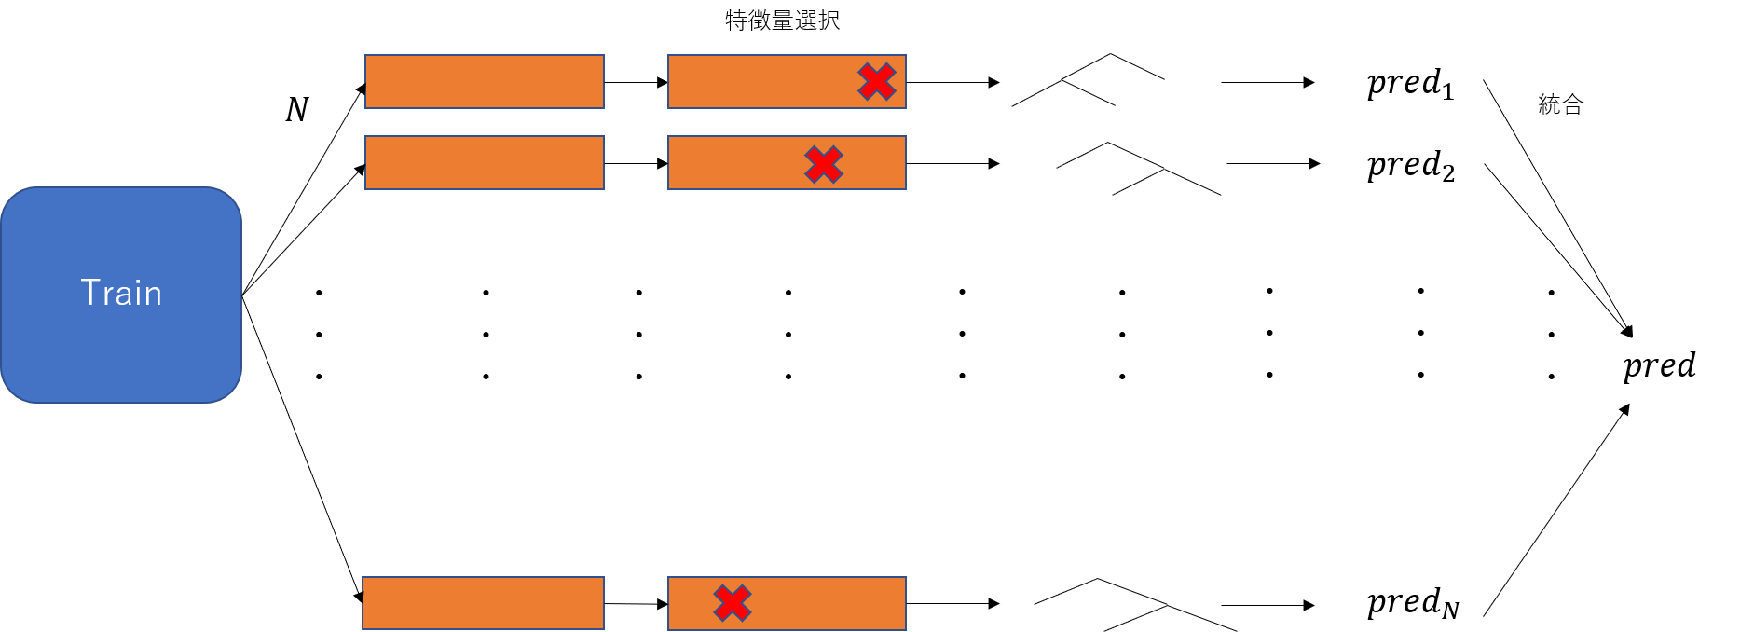
\includegraphics[scale=0.5]{./images/RFR.pdf}
\caption{ Random Forest Regression の内部処理を図式化したもの}
\label{fig:ex1_I_1}
\end{figure}

\texttt{sklearn.linear\_ensemble.RandomForestRegressor}におけるパラメータおよびその意味は,以下である。~\cite{sklearn_RFR}

\begin{itemize}
\item \textit{n\_estimators}\\
これはバギングに用いる木の数である。この数は最適化する必要があると考えた。
\item \textit{criterion}\\
 \textit{criterion} はデータを分割する際の指標であり,不純度を評価している指標である。不純度が大きいことは分割したデータがあるクラスに偏っていることを意味し,不純度が小さくなるように分割する必要がある。このパラメータは \textit{mse} または \textit{mae} のどちらかをとるが,本課題では default である \textit{mse} を用いた。
\item \textit{max\_depth}\\
これは決定木の深さを調節するパラメータである。この値を最適化するよりは後述する\\ \textit{min\_samples\_split} の最適化を行うことで overfitting 等の抑制を行うこととしたため, default でもある \textit{None} とした。
\item \textit{min\_samples\_split}\\
これはノードを分割するために必要な最小サンプル数である。過学習を防ぐ必要もあり,最適化する必要があると考えた。
\item \textit{min\_samples\_leaf}\\
これはノードを構成するために必要な最小サンプル数であり,仮に \textit{min\_samples\_split} が 5 であり,分割する前のノードに 5 つサンプルが含まれていたとしても, \textit{min\_samples\_leaf} が 3 であれば分割できないことになる。この値も最適化する必要があると考えた。
\item \textit{min\_weight\_fraction\_leaf}\\
これはノードの重みの総和に対する最小の重みの割合を考える指標であり,この値を設定すると少なくとも \textit{min\_weight\_fraction\_leaf} より大きな重みが必要であるということになる。このパラメータは重要性が低いと考え,最適化を行わず default の $0.0$ とした。
\item \textit{max\_features}\\
これは最適な分割を行うために考慮すべき特徴量の数を指定するパラメータであり,取り得るパラメータは \textit{auto}(\textit{i.e.} 全ての特徴量を使う。),\textit{sqrt}(\textit{i.e.} $\sqrt{(全特徴量の数)}$を使う。),\textit{log2}(\textit{i.e.} $\log_2{(全特徴量の数)}$を使う。),int (\textit{i.e.} int を使う。), float (\textit{i.e.} (全特徴量の数)$\times$ float を使う。)である。このパラメータは最適化する必要があると考え,本演習では float を指定した。
\item \textit{max\_leaf\_nodes}\\
これは最大のノードの数である。 default では \textit{None} であるが,過学習の抑制のため最適化することとした。
\item \textit{min\_impurity\_decrease}\\
この値は決定木の成長を停止するための閾値となる値であり,不純度がこれより小さくなると分割を停止するというものである。以下の計算式で表されるパラメータとなっている。\\
\linebreak
$\frac{N_t}{N\times (impurity - \frac{N_{tR}}{N_t} \times (right\_impurity) - \frac{N_{tL}}{N_t} \times (left\_impurity))}$\\
\linebreak
$N$はサンプル数,$N_t$は現在のノードのサンプル数,$N_{tR}$は右側の子ノードのサンプル数,$N_{tL}$は左側の子ノードのサンプル数を表しており, $impurity$ は不純度である。本演習ではノードの数やノード内のサンプル数等で過学習を抑制するため,この値まで最適化する必要性がないと判断し, default である 0 を用いた。
\item \textit{boot\_strap}\\
これは木を作成する際にブートストラップを用いるか否かの指標であり,\textit{True} とした。
\item \textit{oob\_score}\\
\textit{oob} とは out of bag の略であり,各 bootstrap においてサンプリングされなかったサンプルを指す。これを学習の正確度計算に用いるか否かの指標となっており,本課題では \textit{True} とした。 
 
\item \textit{warm\_start}\\
これは Lasso 回帰同様,前回学習させた学習器の情報を再利用するか否かの指標であり,本課題では平等に評価を行うために \textit{False} とした。

\item \textit{ccp\_alpha}\\
\textit{ccp} とは cost-complexity pruning の略である。木は大きく複雑であるほど誤分類を防ぐことができる一方で汎化性能が低下してしまう。そのためこの \textit{ccp\_alpha} とノードの数の乗算値を罰則項として用いることで,木の刈り込みを行うというものである。最適化する必要があると考えた。なお,効果的な $\alpha$ は以下のように定義されていた。\cite{ccp}\\
\linebreak
$$\alpha_{eff}(t) = \frac{R(t) - R(T_t)}{|T| - 1} \eqno(2)$$\\
\linebreak

ここで$R(t)$は刈り込み後の誤分類の数,$R(T_t)$は刈り込み前の誤分類の数,$|T|$は決定木の大きさを表す。

\item \textit{max\_samples}\\
ブートストラップを行う上でサンプル数の最大数を指定するものであるが,サンプル数を制限することによる本演習における有用性が感じられず, default である \textit{None} とした。
\end{itemize}

以上より,最適化するハイパーパラメータは \textit{n\_estimators} , \textit{min\_samples\_split} , \textit{min\_samples\_leaf} , \textit{max\_features} , \textit{max\_leaf\_nodes} , \textit{ccp\_alpha} の6つとした。\\

\subsubsection{各ハイパーパラメータの探索範囲}
\begin{itemize}
\item \textit{n\_estimators}\\
木の数が多ければ多いほど,バリアンスを低くすることはできる可能性があるが,トレードオフの関係であるバイアスに影響を及ぼしてしまう。今回は default 値の100 よりは大きな値を探索する一方で,大きすぎてはいけないことから探索範囲を 100 から 1000 とした。
\item \textit{min\_samples\_split}\\
この値は最小で 2 であるが,どこまで大きな値を取れば良いかを考える際に,2 つに均等に分類されたときの一方のノードのサンプル数が 10 より大きいとまだ分類の余地があるのではないかと考えたため,最大値は$2 \times 10$,すなわち探索範囲は 2 から 20 とした。
\item \textit{min\_samples\_leaf}\\
上述した通り,一方のノードのサンプル数 10 より大きいとまだ分類の余地があると考えたため,探索範囲は 1 から 10 とした。
\item \textit{max\_features}\\
必要な特徴量の数は,半分は必要ではないかと考え, float で 0.5 から 1.0 とした。
\item \textit{max\_leaf\_nodes}\\
訓練データは約 1200 個である。そのためノードの数はそれよりも小さくなるはずであり,1200に近い値であると過学習の恐れがあるため最大値を 1000 とし,最小値は 100 としてこの範囲で探索を行った。\\
\item \textit{ccp\_alpha}\\
(2) より効果的な $\alpha$ を考えると,決定木のサイズが大まかに $1000$ であると仮定し,分子が最小で $1$ であることを考慮すると,最適な値は 1e-3 あたりでないかと考える。概算した結果を含んだ範囲を探索するように,1e-5から1e-1までを探索することとした。
\end{itemize}

\subsubsection{ハイパーパラメータ探索方法} 
 Lasso 回帰同様にハイパーパラメータ探索には optuna ~\cite{optuna}を用いて, cross validation における RMSE 値の平均をとり,その値が最小となるように100回探索を行った。

 \textit{n\_estimators} は int 指定で 100 - 1000, \textit{min\_samples\_split} も int 指定で 2 - 20, \textit{min\_samples\_leaf} も int 指定で 1 - 10, \textit{max\_features} は 0.5 - 1.0 の範囲で対数一様分布からサンプリングした値, \textit{max\_leaf\_nodes} は int 指定で 100 - 1000, \textit{ccp\_alpha} は 1e-6 ~-1e-1 の範囲の対数一様分布からサンプリングした値を回帰のパラメータとした。cross validation を行う際には,\\\texttt{sklearn.model\_selection.cross\_val\_score} を用いて,引数には学習器,小分子の説明変数,目的変数,スコアリングには2乗平均平方根誤差の負の値を用いる \textit{neg\_root\_mean\_squared\_error} を使い,cross validation 数は 5 としてスコアを算出した。この返り値は cross validation の数だけ scoring の値が格納された list となるため,optuna において最小化してほしいスコアである RMSE 値となるようにそれらの平均を取り,このままでは負の数であるため -1 をかけることで正の数に変換して optuna で最小化したいスコアである RMSE 値とした。
 
\subsubsection{最良ハイパーパラメータ}
探索を行った7つに対し,最良ハイパーパラメータは以下のようになった。\\
\linebreak
$\textit{n\_estimators} = 460$\\
$\textit{min\_samples\_split} = 2$\\
$\textit{min\_samples\_leaf} = 1$\\
$\textit{max\_features} = 0.6400954926671139$\\
$\textit{max\_leaf\_nodes} = 575$\\
$\textit{ccp\_alpha} = 1.0658736175592873$e-$05$\\

\subsubsection{最良ハイパーパラメータにおける cross validation 中の $\ln{K_a}$ 値の RMSE と $\ln{K_a}$ 値の相関係数 R}
 cross validation 中の $\ln{K_a}$ 値の RMSE 並びに $\ln{K_a}$ 値の相関係数 R を以下に示す。なお,最良パラメータを用いるには optuna の Attributes の 1 つである \texttt{best\_params} を利用する。この Attribute の返り値は dictionary であるため,回帰のパラメータとして用いるにはアンパックを行うため \texttt{**} をつける必要がある。また cross validation を行うため \texttt{skleran.model\_selection.KFold} を用いた。\texttt{KFold.split()} の引数に訓練データの説明変数,目的変数を入れ,繰り返し処理を行うことで cross validation が実行される。この際, \texttt{KFold.split()} では index が取得できるため,繰り返し処理内で訓練データのインデックスを指定して,さらに訓練データと検証データに分割し, validation を行う。学習結果は \texttt{sklearn.metrics.mean\_squared\_error} の引数に検証データの目的変数と予測値を指定して計算した後,平方根を取れば RMSE を求めることができる。また, \texttt{numpy.corrcoef()} メソッドの引数に同じく検証データの目的変数と予測値を指定すると分散共分散行列が計算されるため,非対角成分を取得することで相関係数 R を求めることもできる。以上のプロセスをリストに都度追加していき, cross validation が終了したのちにリストを出力することで値を得ることができる。\\
\begin{itemize}
\item  cross validation 1\\
RMSE $= 0.4644035832147438$\\
R $= 0.7889564461816483$ \\
\item  cross validation 2\\
RMSE $= 0.4427123851402675$\\
R $= 0.7880714111267291$ \\
\item  cross validation 3\\
RMSE $= 0.37761214578583624$\\
R $= 0.8132106435791429$ \\
\item  cross validation 4\\
RMSE $= 0.43001360403166555$\\
R $= 0.8070416146526004$ \\
\item  cross validation 5\\
RMSE $= 0.42854181803491354$\\
R $= 0.8117764861589346$ \\
\end{itemize}


\subsection{Cyclic peptide drug の予測における $\ln{K_a}$値の RMSE , $\ln{K_a}$ 値の相関係数 R}
 選択されたハイパーパラメータを用いて Small molecule データを教師データとした Random Forest 回帰でCyclic peptide drug の予測を行なった結果を以下に示す。なお,この際に用いる教師データは Small molecule 全体であるため,学習器には Small molecule 全体のデータを用いる必要がある。また, RMSE および R を求めるには cross validation 内で行ったことと同じプロセスを辿れば良い。\\
 \linebreak
RMSE $= 0.6531016693402263$\\
R $= 0.5388666099065988$ \\
%I-E==========================================================================================

%I-H============================================================================================
\subsection{重要な記述子についての考察}
重要な記述子を \texttt{sklearn.ensemble.RandomForestRegressor.feature\_importances\_} において値が$0.02$より大きいものであると定義する。その時,重要な記述子は RDKit の 2D descriptors $208$ の内,$7$に絞られた。それらを大きいものから順に示す。なお,出力する際には 2D 記述子のリストを予め取得しておき, \texttt{sklearn.ensemble.RandomForestRegressor.feature\_importances\_} を \texttt{zip} で繰り返し処理を行い,importance が 0.02 より大きい場合に出力するようにすれば良い。\\
\begin{itemize}
\item  \textit{MolLogP} (importance : $0.310359580332063$) \\
 \textit{MolLogP} は Lasso 回帰同様に最も重要な記述子であるということが分かり,脂溶性と血漿タンパク質との結合率 $f_b$ との関係がやはり大きいということが確認できる。
\item  \textit{SMR\_VSA7} (importance : $0.047524561084776436$) \\
 \textit{SMR\_VSA} は先述した MOE 独自の記述子のうち,分子屈折率 (MR) と表面積の寄与を用いた記述子となっており, \textit{SMR\_VSA7} はその値が 3.05 以上 3.63 未満のものを指している。\cite{smr} \cite{smr_vsa}
\item  \textit{BCUT2D\_MRHI} (importance : $0.03212854034578604$) \\
 \textit{BCUT2D} は原子量, Gasteiger 電荷という電子の電気陰性度を基にして決定する点電荷\cite{gas},MolLogP,MolMRを対角成分としたベクトルで,それぞれの固有値の最大値と最小値が要素となっている。\cite{BCUT2D}
 \textit{BCUT2D\_MRHI} は MR の最大固有値を指している。
\item  \textit{SlogP\_VSA6} (importance : $0.03018716865299929$) \\
 \textit{SlogP\_VSA} は先述した MOE 独自の記述子のうち,$\log{P}$ の値と表面積の寄与を用いた指標となっており, \textit{SlogP\_VSA6} はその値が 0.15 以上 0.20 未満のものを指している。 \cite{smr} \cite{smr_vsa}
\item  \textit{PEOE\_VSA6} (importance : $0.02604793965526905$) \\
 \textit{PEOE\_VSA} は MOE 独自の記述子のうち,部分電荷と表面積の寄与を用いた記述子となっており, \textit{PEOE\_VSA6} はその値が $-$0.10 以上 $-$0.05 未満のものを指している。\cite{smr} \cite{smr_vsa}
\item  \textit{SMR\_VSA10} (importance : $0.02151527420149223$) \\
 \textit{SMR\_VSA10} は,先述した \textit{SMR\_VSA} の値が 4.00 以上のものを指している。\cite{smr} \cite{smr_vsa}
\item  \textit{VSA\_EState6} (importance : $0.021178404488366054$) \\
 \textit{VSA\_EState6} は先述した \textit{VSA\_EState} の値が 6.00 以上 6.07 未満 のものを指している。\cite{estate_vsa}
\end{itemize}

以上の記述子より, Random Forest Regression において Lasso 回帰と異なる重要な記述子の多くは,分子屈折率や電荷に関するものであった。すなわち血漿タンパク質との結合率 $f_b$ が分子屈折率と関係がある一方で,その関係は線形関係ではないために Lasso 回帰では重要視されなかった可能性が考えられる。このことは bin が最大の場合や最小の場合以外にも重要度が大きい記述子があることからも示唆される。また VSA 記述子の重要度が高くなっており,表面積あたりの特性が予測精度に関与している可能性が高いと考える。

\subsection{目的変数を変えた時の予測精度の比較・考察}
予測精度は Cyclic peptide drug を目的変数としたときの方が Lasso 回帰同様に低かった。なお Lasso 回帰の場合と異なり,並外れた値ではなかったが,同じ修正を施したもので計算を行っても予測精度が上がることはなかった。結果を以下に示す。\\
\linebreak
RMSE $= 0.6450219425012329$\\
R $= 0.5299471326326767$ \\

真値との差が1より大きかったものが以下の2分子である。\\

\begin{figure}[H]
\centering
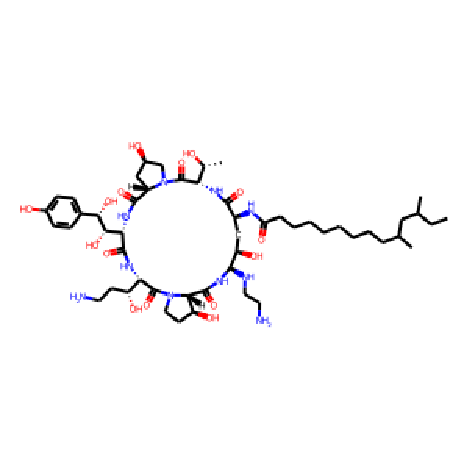
\includegraphics[scale=0.5]{./images/Caspofungin.pdf}
\caption{Caspofunginの構造式出力}
\label{fig:ex1_I}
\end{figure}
$true - pred = 1.4978040040756992$
\begin{figure}[H]
\centering
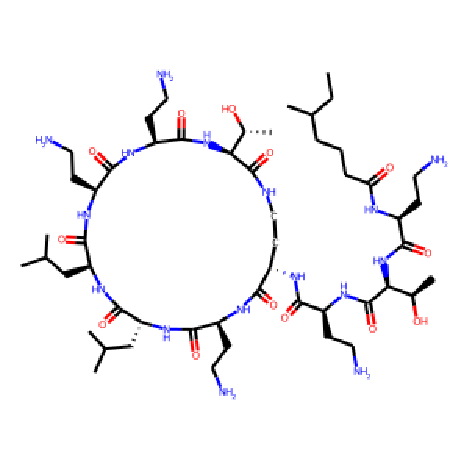
\includegraphics[scale=0.5]{./images/Colistin.pdf}
\caption{Colistinの構造式出力}
\label{fig:ex1_I_2}
\end{figure}
$true - pred = 1.2772413714104842$\par
一方で真値との差が0.1より小さかったものが以下の2分子である。
\begin{figure}[H]
\centering
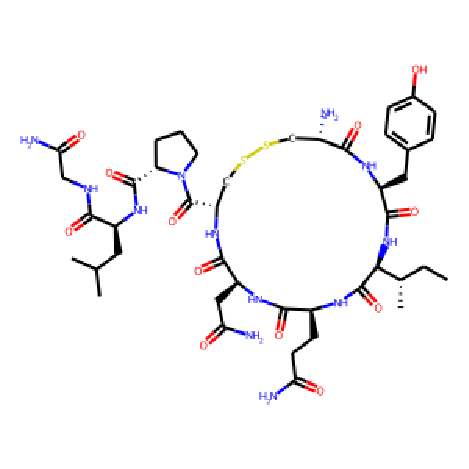
\includegraphics[scale=0.5]{./images/Oxytocin.pdf}
\caption{Oxytocinの構造式出力}
\label{fig:ex1_I_3}
\end{figure}
$true - pred = -0.028241018662841177$
\begin{figure}[H]
\centering
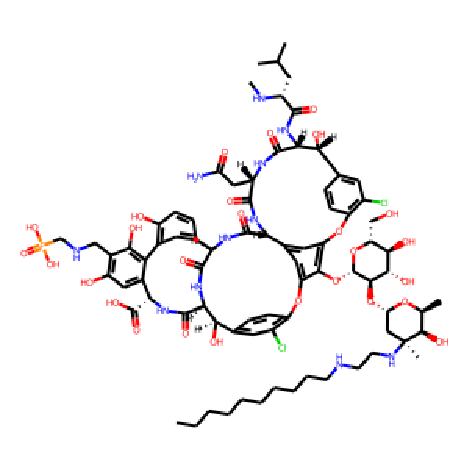
\includegraphics[scale=0.5]{./images/Telavancin.pdf}
\caption{Telavancinの構造式出力}
\label{fig:ex1_I_4}
\end{figure}

$ true - pred = -0.002621245656653448$\par

これらの違いを構造式から確認することが困難であったため,それぞれの記述子の値を比較し,前者と後者でやや値に差が見られたものについてその記述子と値の一部を示す。なお,ここでの差は統計的に有意なものを確かめたのではなく,主観的なものとなっている。
\begin{itemize}
\item  \textit{BCUT2D\_MWHI}\\
Caspofungin:16.33303999707714,Colistin:16.274319729818163\\
Oxytocin:33.11460794525803,Telavancin:35.49679579150821\\
\item  \textit{BCUT2D\_MRHI}\\
Caspofungin:5.979840534258863,Colistin:5.979840534258863\\
Oxytocin:8.763128354458999,Telavancin:7.5119995728238464\\
\item  \textit{SMR\_VSA10}\\
Caspofungin:41.35025810546054,Colistin:64.97897702286656\\
Oxytocin:86.56677297564003,Telavancin:78.11720550066529\\
\item  \textit{SlogP\_VSA12}\\
Caspofungin:0.0,Colistin:0.0\\
Oxytocin:21.587795952773448,Telavancin:30.79764210725292\\
\end{itemize}

\par\textit{BCUT2D\_MWHI} と \textit{BCUT2D\_MRHI} が後者 2 分子において値が大きいことは,それぞれの最大固有値がより大きく,情報を多く含んでいる分子の方が予測精度が高いことを意味している。また \textit{SMR\_VSA10} や  \textit{SlogP\_VSA12} はそれぞれの指標の bin において無限大を含む指標になっている(\textit{i.e.} 上限がない)。VSA は先述したようにある一定範囲の分子の表面積を記述子としたものであることから,テストデータ内の一部の分子の記述子の値を見た限りでは,ある表面積の大きさ内の特性だけでなく,表面積自体と予測精度が関係しているのではないかと考える。\\

\section{2-c) 予測精度の向上のために行ったこと}
予測精度の向上のため,用いる記述子について考えた。その際,記述子の最適化による予測精度の向上が見られたという論文があった。\cite{qsar}この論文を参考にし,実装を試みたものを以下に示す。
\begin{itemize}
\item  Dragon 7.0 \cite{dragon}の利用\\
\item  CORALSEA \cite{coral}の利用\\
\item  Random Forest Regression における重要度に基づいて記述子を絞り込む\\
\end{itemize}

\subsection{Dragon 7.0 の利用}
Dragon 7.0 は 2D 分子記述子の 1 つであり,RDKit 以外の記述子も論文で用いられることが多いことがわかった。しかしながら, Dragon 7.0 はサービスが終了しており,実装が困難であったため,他の分子記述子を用いることを試みた。 論文内でも Dragon にはある記述子の計算ができないといった旨が記されており,そのような不具合を解消した分子記述子計算ソフトウェア mordred \cite{mordred}というものを用いることにした。使用の際には,\texttt{mordred} から \texttt{Calculator} , \texttt{descriptors} をインポートすることで利用できる。\texttt{Calculator(descriptors)} にて計算機のインスタンスを作成し,そのインスタンスの引数に SMILES 式をとることで分子記述子がおよそ1600 - 1800 個計算される。しかしながら,このソフトウェアは不完全であり,一部エラーとなっている記述子が存在する。そのためエラーとなる記述子は説明変数から排除した。さらに \textit{bool} 値の分子記述子も存在し,その場合は \textit{True} ならば 1, \textit{False} ならば 0 とした。\par
検証のため,課題 1 で最適化したハイパーパラメータで Random Forest 回帰を行ったが,検証できなかった。分子によって計算できる記述子が異なるため,説明変数の大きさが一致していないのではないかと考えた。活用には時間を要すると考え,実装は断念した。

\subsection{CORALSEA の利用}
CORALSEA という SMILES 式から 最適な記述子の計算を行うソフトウェアがある。論文内では正しい正規化のために用いられており,こちらの利用も検討したが,ソフトウェアの動かし方の理解に時間を要すると考え断念した。

\subsection{ Random Forest Regression における重要度に基づいて記述子を絞り込む}
簡単な検証のため,課題 1 で \texttt{feature\_importances\_} Attribute を用いて,重要度が0.01より大きくなった記述子13 個のみを用いて RMSE, R を計算した。この検証では,重要度の高い記述子のインデックスを取得し,関数内で逐一インデックスを指定するという非効率的な方法で実装した。結果を以下に示す。\\
\linebreak
RMSE $= 0.6479761913510614$\\
R $= 0.547988855813419$ \\
\linebreak
なお,記述子を絞り込む前の結果を再度示す。\\
\linebreak
RMSE $= 0.6450219425012329$\\
R $= 0.5299471326326767$ \\
\linebreak
比較すると,RMSE 値は精度が低下しているが,R 値は向上している。そのため,記述子を絞り込むという方法は有効である可能性が高いと考えた。\par
論文内では,標準偏差が0の記述子や別の記述子とのピアソン相関係数が 0.95 を上回るような記述子を取り除くということを行っていた。また,R のパッケージを用いて,Random Forest を適用し,設定した閾値を下回る重要度の変数を除いていくということも行なっていた。\par
本課題では,標準偏差が0の記述子を取り除くという点と,設定した閾値を下回る重要度の変数を取り除くという点の実装を行った。なお,モデルは課題1 で最適化したものを利用した。\par
まず,Small molecule データを行列化した訓練データにおいて,列ごとに標準偏差を計算し,値が0となるもののインデックス,すなわち列番号を格納しておく。その列を削除していくが,この際に列番号の小さいものから削除した場合にはずれが生じてしまう。そのため列番号の大きいものから削除していくことでエラーを防いだ。学習後に\texttt{feature\_importances\_}を用いて重要度を計算する。今回設定した閾値の値は 0.01 であるため 0.01 を下回る列番号を格納しておき,標準偏差の場合同様に列を削除していく。一方で削除する列がない場合には全ての重要度が閾値以上であることを意味するため,繰り返し処理を止め,予測精度を計算・出力するようにした。結果を以下に示す。\\
\linebreak
RMSE $= 0.6383771362346949$\\
R $= 0.5433755466603287$ \\
\linebreak
記述子を絞り込む前よりも RMSE,R 共に精度は僅かに上昇した。一方で期待したほどの上昇ではなかった。ここでパラメータの 1 つである \textit{warm\_start} を \textit{True} とすることで前回の学習を利用し,より精度の高い学習ができるのではないかと考え実装した。結果を以下に示す。
\linebreak
RMSE $= 0.6408462854827193$\\
R $= 0.560401097512674$ \\
\linebreak
相関係数 R は僅かに上昇し,今回のように繰り返し処理で学習器を更新していく際には用いた方が良いと分かった。\par
本課題では,主成分分析や論文内で行われていた相関係数,独立性の検定に基づいた記述子の絞り込みを行っていないため,その点を行うことで僅かに精度が上昇する可能性がある。また,RDKit の 2D 記述子は総数 208 であり,論文内で用いられた Dragon よりも少なく,使用できなかった mordred と比較しても少ない。そのため記述子の絞り込みによる効果が十分に発揮されなかったと考える。また,記述子の取捨選択を行なったのちにハイパーパラメータの探索を行っておらず,最適なパラメータとなっていない可能性もあるため,パラメータの探索を行うことで精度が上昇すると考えられる。\par
また,論文内では pH が 7.4 におけるイオン状態を考慮したり,Plasma Protein Binding 値は \textit{in vivo} で算出されたもののみを利用するなど行っていた。さらに,非結合率 $f_u$ を指標としており,結合率だけでなく非結合率も考えることで予測精度が上昇するのではないかと考えた。

\begin{thebibliography}{50}
\bibitem{paper1_Tajimi} Takashi Tajimi \textit{et al.} "Computational prediction of plasma protein binding of cyclic peptides from small molecule experimental data using sparse modeling techniques", \textit{BMC Bioinformatics} \textbf{19}(Suppl 19): 527, 2018. doi: 10.1186/s12859-018-2529-z.

\bibitem{C_previous} IngleBL \textit{et al.} "Informing the human plasma protein binding of environmental chemicals by machine learning in the pharmaceutical space: applicability domain and limits of predictability." \textit{JChem Inf Model}. 2016;56(11):2243-52.

\bibitem{sklearn_Lasso} sklearn.linear\_model.Lasso \\URL : \url{https://scikit-learn.org/stable/modules/generated/sklearn.linear_model.Lasso.html}(アクセス日:2021/5/21).

\bibitem{optuna} Optuna \\URL : \url{https://optuna.org}(アクセス日:2021/5/21).

\bibitem{git_ipc} IPC Descriptor gives suspiciously large values  \\URL : \url{https://github.com/rdkit/rdkit/issues/1527}(アクセス日:2021/5/24).

\bibitem{rdkit_mollogp} rdkit.Chem.Crippen module  \\URL : \url{https://www.rdkit.org/docs/source/rdkit.Chem.Crippen.html}(アクセス日:2021/5/23).

\bibitem{logp} ケモインフォマティクスとLogP計算:CLogPのCは"calculated"ではありません \\URL : \url{https://future-chem.com/logp/}(アクセス日:2021/5/23).

\bibitem{mollogp} Scott A. Wildman \textit{et al.} "Prediction of Physicochemical Parameters by Atomic Contributions", \textit{Journal of Chemical Information and Computer Sciences} \textbf{39}: 868-873, 1999. doi: 10.1021/ci990307l.

\bibitem{fp} RDKitでフィンガープリントを使った分子類似性の判定\\URL :  \url{https://future-chem.com/rdkit-fingerprint/}(アクセス日:2021/5/23).

\bibitem{fp_source1} rdkit/rdkit/Chem/Descriptors.py \\URL : \url{https://github.com/rdkit/rdkit/blob/master/rdkit/Chem/Descriptors.py}(アクセス日:2021/5/23).

\bibitem{fp_source2} rdkit/rdkit/Chem/Draw/SimilarityMaps.py \\URL : \url{https://github.com/rdkit/rdkit/blob/c2fb57c19f8bac4aac07f4d0915ece8d95f7c963/rdkit/Chem/Draw/SimilarityMaps.p}(アクセス日:2021/5/23).

\bibitem{fp_ID} 【RDKit】Morganフィンガープリントの生成ルールを解釈してみた \\URL : \url{https://qiita.com/oki_kosuke/items/9a7b52911c4ef9d4edad}(アクセス日:2021/5/23).

\bibitem{hallkier} R\'{e}ka Laczk\'{o}-Rig\'{o} \textit{et al.} "Structural dissection of 13-epiestrones based on the interaction with human Organic anion-transporting polypeptide, OATP2B1", \textit{The Journal of Steroid Biochemistry and Molecular Biology} \textbf{200}: 2020. doi: 10.1016/j.jsbmb.2020.105652.

\bibitem{fr} Electronic Supplementary Material (ESI) for CrystEngComm. \\URL : \url{http://www.rsc.org/suppdata/ce/c4/c4ce01912a/c4ce01912a1.pdf}(アクセス日:2021/5/23).

\bibitem{plusma} 血液成分であるタンパク質の種類について【電気泳動による血清タンパク分画による分類】\\URL : \url{https://totthi.com/blood-component/}(アクセス日:2021/5/23).

\bibitem{moa_vsa} MOE/ケモインフォマティクス \\URL : \url{https://www.molsis.co.jp/lifescience/moe/qsar/}(アクセス日:2021/5/23).

\bibitem{estate_vsa} rdkit.Chem.EState.EState\_VSA module \\URL : \url{http://rdkit.org/docs/source/rdkit.Chem.EState.EState_VSA.html}(アクセス日:2021/5/23).

\bibitem{qed} RDKitで薬らしさを定量的に評価する \\URL : \url{https://future-chem.com/rdkit-qed/}(アクセス日:2021/5/23).

\bibitem{RF} ランダムフォレスト (Random forest) とは?機械学習モデルを分かりやすく解説!! \\URL : \url{https://nisshingeppo.com/ai/random-forest/}(アクセス日:2021/5/24).

\bibitem{sklearn_RFR} sklearn.ensemble.RandomForestRegressor \\URL : \url{https://scikit-learn.org/stable/modules/generated/sklearn.ensemble.RandomForestRegressor.html}(アクセス日:2021/5/24).

\bibitem{ccp} 1.10. Decision Trees \\URL : \url{https://scikit-learn.org/stable/modules/tree.html}(アクセス日:2021/5/24).

\bibitem{smr} ChemDes/MOE-type descriptors (60) \\URL : \url{http://www.scbdd.com/chemdes/list10/}(アクセス日:2021/5/25).

\bibitem{smr_vsa} rdkit.Chem.MolSurf module \\URL : \url{http://rdkit.org/docs/source/rdkit.Chem.MolSurf.html}(アクセス日:2021/5/26).

\bibitem{gas} 佐々木皓平 他 . 高精度な分子動力学計算のための静電相互作用パラメータの検討 \\URL : \url{http://www.molsci.jp/2018/pdf/1P103_m.pdf}(アクセス日:2021/5/26).

\bibitem{BCUT2D} rdkit.Chem.rdMolDescriptors module \\URL : \url{http://rdkit.org/docs/source/rdkit.Chem.rdMolDescriptors.html}(アクセス日:2021/5/26).

\bibitem{qsar} Cosimo Toma \textit{et al.} "QSAR Development for Plasma Protein Binding: Influence of the Ionization State", \textit{Pharmaceutical Research} \textbf{36}: 28, 2019. doi: 10/1007/s11095-018-2561-8.

\bibitem{dragon} Kode. Dragon (Software for Molecular Descriptor Calculation) version 7.0. Kode srl; 2016.

\bibitem{coral} CORAL-QSAR/QSPR \\URL : \url{http://www.insilico.eu/coral/}(アクセス日:2021/5/27).

\bibitem{mordred} 森脇寛智 \textit{et al.} "分子記述子計算ソフトウェア mordred の開発", ケモインフォマティクス討論会 39, 2016. doi: 10.11545/ciqs.2016.0\_Y4.
% \bibitem{Kanaoka2010} 金岡晃,島岡政基,岡本栄司.IDベース暗号の信頼構築フレームワーク, 情報処理学会論文誌,51(9),1692-1701 (2010)
% \bibitem{Mirakhorli2016} M. Mirakhorli, J. Cleland-Huang. Detecting, Tracing, and Monitoring Architectural Tactics in Code, IEEE Transactions on Software Engineering, 42(3), 206-220 (2016)
% \bibitem{Chiba1990} 千葉則茂, 村岡一信.レイトレーシングCG入門, Information \& Computing, vol. 46, サイエンス社 (1990)
% \bibitem{KR1989} B.W. カーニハン, D.M. リッチー(石田晴久訳).プログラミング言語C 第2版 ANSI規格準拠,共立出版 (1989)
%\bibitem{texLecture}  情報リテラシ第二 テーマ2 科学技術文書執筆\url{https://titechcomp.github.io/y19-il2j/theme2.html}(アクセス日:2020/6/10)
% \bibitem{Okumura1991}奥村晴彦.C言語による最新アルゴリズム事典,技術評論社 (1991)
\end{thebibliography}
\end{document}